%
% RING Meeting Template
% Edit and compile with pdflatex
%
% If you absolutely want to use latex to produce DVI, be sure to use only
% compatible graphisms (.eps is the best).
% You can also include .eps figs only and use pdflatex (thanks to epstopdf),
% just check that you have "shell_escape = 1" somewhere in a texmf.cnf file,
% or that you call "pdflatex -shell-escape file.tex".
%
% This template uses natbib.sty bibliography style, so you can use commands
% like \citet{}, \citep{}, \citeauthor{} or \citeyear{}.

%-----------------------------------------
% Template Mode preprint / final:

%\documentclass[preprint]{ring20} 

% Please : submit your paper in the final mode
\documentclass[final]{ring20} 

%% relative path to the graphic folder from the tex file
\graphicspath{%
{./Figures/}%
}

%-----------------------------------------
% First page information :

\title{Progresses in the implicit structural modeling benchmark}

% Title used for the title over-riding report
% (It may be the same than the main title if small enough)
\shorttitle{Implicit structural modeling benchmark}

% Author(s) name(s) on the first page
\author[1]{Guillaume Caumon}
\author[1,2]{Julien Renaudeau}
\author[1]{Modeste Irakarama}
\author[3]{Lachlan Grose}
\author[5]{Miguel de la Varga}
\author[7]{Michael Hillier}
\author[7]{Eric de Kemp}
\author[5]{Florian Wellmann}
\author[1]{Pauline Collon}
\author[4]{Gautier Laurent}
\author[3]{Laurent Ailleres}
%\author[8]{Who else ? Order to be determined}

%Adresses of the authors (affiliations)  
\affil[1]{RING, GeoRessources / ENSG, Universit\'e de Lorraine / CNRS, France}
\affil[2]{Schlumberger, France}
\affil[3]{Monash University, Australia}
\affil[4]{Univ. Orl\'eans, CNRS, BRGM, ISTO, France}
\affil[5]{RWTH Aachen, Germany}
\affil[6]{BRGM, France}
\affil[7]{NRCan, Canada}


%often used affiliations
%\affil[1]{GeoRessources - UL/CNRS/CREGU, ENSG, Vandoeuvre-l\`es-Nancy, France.}
%\affil[2]{GeoRessources - UL/CNRS/CREGU, ENSMN, Nancy, France.}
%\affil[3]{Centre d'hydrog\'eologie et de g\'eothermie, Universit\'e de Neuchatel, Neuchatel, Suisse.}
%\affil[5]{INRIA - Project Alice, Villers-l\`es-Nancy, 54600, France.}

% Author(s) name(s) used in the footer of each page
\shortauthor{Caumon et al.}

%-----------------------------------------
% The document :
%

\begin{document}
\maketitle

\begin{abstract}

Implicit methods have gained significant popularity in recent years as 
an alternative to surface-based structural modeling methods (also known as 
contouring, gridding or explicit structural modeling). These approaches represent 
geological interfaces as equipotentials of a scalar field. 
Whereas existing formulations share the same principle, they have not yet been 
quantitatively compared beyond theoretical discussions. In this paper, we review 
the main categories of implicit methods and list their parameters. We propose 
three benchmark data sets: a folded turbidite, a carbonate buildup 
displaying large thickness variations and a convoluted synthetic surface 
representing a hydrothermal body. We applied several methods and several 
implementations on these data sets, and provide the chosen parameters for each 
methods. Results are compared in terms of accuracy, ability to predict 
some features not present in the data, and topological complexity. 
Results illustrate the difficulty to come up with a universal geological 
modeling method, and highlight the need to build additional geological 
knowledge and to consider uncertainty in future structural modeling methods.  

\end{abstract}

\todo[inline]{Writing mode: I suggest a ``dictatorial collaborative writing'': co-authors send me comments / paragraphs / figures / results in annotated PDFs, LateX (or Word) format and I will incorporate them in the LaTeX document.

Authors: list and order to be discussed. }


\todo[inline]{Eric: "I was thinking of developing  further a 3d matrix with principal axis indicating model  level of complexity (dimension+properties, geological events, cumulative spatial features) as well as a matrix indicating data complexity (density, number of types, clustering)  . Each test case could fit into these two matrices and could be increased in dimensionality but is at least more intuitive where the case examples fall visually. Each case would get a complexity badge or glyph classifying it."}

\textit{This paper an update from the 2019 RING Meeting version. It includes the first results from 6 different implicit modeling codes.}

\section*{Introduction}

The formation and deformation of rocks at geological time scales generate a large variety of geological structure shapes. Three-dimensional structural modeling aims at reconstructing these structures from spatial samples created from field observations and/or from geophysical images of the subsurface. Historically, structural modeling first meant computing the depth contours of a particular geological interface \citep[e.g.,][]{Walters1969AB,Hardy1971JGR,Briggs1974G,Bolondi1976G}. During the 1990's surface-based models using polygonal or parametric surfaces emerged as a more powerful way to represent complex structures such as recumbent folds or salt diapirs \citep{Mallet1992CD,deKemp1999CG}. However, these explicit modeling approaches are difficult to automate in complex geological settings, and call for various degrees of interactive input to generate the structures. Since then, progress in memory and computational capabilities have led to implicit modeling formulations, in which geological interfaces between rock units are defined by isovalues of a three-dimensional scalar field \citep{Lajaunie1997MG,Cowan2002ASGMEM,Calcagno2008PEPI,Frank2007CG,Caumon2013GaRSITo,Souche20137ECEISE2,Hillier2014MG,Laurent2016MG,Laurent2016EaPSL,Martin2017CG,Grose2017JSG,delaVarga2018GMDD,Irakarama2018EAGE,Grose2019JoSG,Renaudeau2019BEMRMX,Renaudeau2019MG,Manchuk2019C&G}.

Implicit modeling provides a high degree of automation even for complex geological shapes, and can also account for various types of structural data such as off-contact orientation  measurements. As a result of these methodological advances, three-dimensional structural modeling is increasingly becoming part of the geologist's toolbox. By integrating sparse data into a consistent graphical model, the promise of computational structural modeling is to help geologists to analyze their data, to develop conceptual interpretive models, and to make subsurface forecasts based on model outcomes. 

Automation of three-dimensional structural modeling is essential to meet these needs effectively, especially when several possible models need to be considered to appropriately characterize subsurface uncertainty \citep{Wellmann2018AiG}. However, ``seeing is believing'', so a risk is that applied geologists believe that a particular structural model is true, whereas it is only determined from the available spatial data (whose reliability may vary) and from mathematical or numerical terms telling what the three-dimensional model should look like away from the data points. Indeed, in general, the data points are not numerous enough to fully characterize the structural geometry, hence the need for some sort of regularization \citep[e.g.,][]{Renaudeau2019MG}. The parameters involved in the regularization term influence the results, but may not be easy to determine by layman users. These parameters oftentimes correspond to abstract mathematical terms (e.g., least-squares weights, variogram ranges, basis function parameters) which can be intuitively translated into model features (e.g., degree of data fit, stiffness of the surface) but not so easily into classical structural concepts, which generally involve a blend of geometric, kinematic, and mechanical reasoning. Analyzing and understanding the results of a particular method can be difficult, as it may call for the practitioner to delve into the theory of partial differential equations, numerical optimization, or geostatistics. 

To address these challenges, several authors have proposed to more directly integrate structural concepts into modeling methods \citep{DeKemp2003G,Maxelon2009C&G,MassiotGM2010,Laurent2016EaPSL,Grose2017JSG,Grose2018JGRSE,Grose2019JoSG}. This can be achieved either by manually or automatically adding new interpretive ``data'' such as fold hinges, or by integrating new mathematical terms in the interpolation problem. Another recent line of research has been on the mathematical formulation and the discretization of the regularization term \citep{Laurent2016MG,Martin2017CG,Irakarama2018EAGE,Renaudeau2019MG}. In this frame, theoretical comparisons between the various published methods can be made, but they may be of limited use to practitioners. Practical comparisons are delicate because they rely on software packages whose implementation is not necessarily available. The level of implementation descriptions may also vary from one paper to another, making it difficult for graduate students to reproduce previous work. 

%However, the choice of a methodology can remain difficult for the practitioner, both the practical and fundamental reasons.  

%Software availablility and usability are important, sability issues, even though they can important, but we will focus on  Among these, the ability of a particular interpolation method to interpolate or extrapolate correct structural geometries away from data points can always be challenged. The adequacy of automatic methods has been debated since the early times of automatic map contouring \citep{Walters1969AB}. The data density should be such that results are well constrained.  ideally, a good method should be able produce results similar to those of a skilled structural geologist.  but this can be difficult to quantify.  . In principle, the goodness of an interpolated structural geometry can be measured on a particular data set by cross-validation (ie: computing the error between the forecasted geometry and some randomly chosen data points). However, as in machine learning, the tuning parameters of a particular method can be optimized using cross-validation, raising the risk of overfitting. Philosophically, 

The goal of this paper is to propose a set of benchmark data sets to compare existing and future structural modeling methods. Similar benchmark data exist in the computer graphics community \citep[e.g.,][]{BLNTS13}, but they generally aim at reconstructing only one single manifold surface from a relatively dense point cloud. In geosciences, the difficulty to access the subsurface generally entails more sparsity and more diversity in the field data. In particular, stratigraphic orientations are often available from fieldwork and dipmeter measurements in boreholes. Another difficulty specific to geological modeling is the presence of faults, and the simultaneous reconstruction of several conformable stratigraphic surfaces with just one scalar field, which raises questions about the management of thickness variation \citep{Laurent2016MG}. The data sets presented in this paper (Section \ref{sec:data}) account for these geological peculiarities and propose several test cases of variable complexity. Each case includes basic data types (points and orientations). To keep the comparison simple, more advanced data types such as fold axis, foliation data, and structural lineations are not considered in the present paper. Some faults are present  in two data sets, but they have limited displacement and so they may be ignored, as fault management in the various techniques is outside the scope of this comparison. 

Before presenting the results, Section \ref{sec:methods} proposes a synthetic review of the various existing methods, and describe, for each method (or computer implementation) used in this benchmark, its main parameters. The three-dimensional models obtained with the various codes are available on a public repository \footnote{\url{https://github.com/Loop3D/ImplicitBenchmark/}}, which make it possible to scrutinize the results and also to add new results or new data sets in the future. In Section \ref{sec:results}, we summarize these results in terms of accuracy, spatial forecasting ability and topological complexity.  

\todo[inline]{I removed the end of the sentence (in terms of quality, accuracy, ability to spatially predict the reference surface away from the data points and computational time) because we cannot fully define these terms here. I also added some precision in the results part. The essential point that needs to be made in the discussion is that honoring some unseen or subtle features calls for parameters whose values must be inferred. So we somehow will need to discuss about model parsimony and ability to integrate prior knowledge which is not directly present in the data.

Previous comments: 

PC: "this supposes there is a "reference true" surface? I do not like it very much... 
Shoudn't we  keep the analysis focused on what we know (data, geological concepts ?). 
In this case, I would prefer "ability to consistently extrapolate the surface"... 

MI: "- What is "quality" in this context and how do we measure it?
- About the ability to predict the reference surface away from data, as we discussed some time ago, I think this is questionable.
  In practice, I can think of two cases: (1) Either we have an a priori on that reference surface away from the data  and therefore we should provide that information to our interpolator.
  Otherwise we know in advance that the interpolator will most likely not predict the surface away from the data because we explicitly ask the interpolator for a "smooth" surface.
  (2) Either we do not have an a priori on that reference surface and therefore we just have to accept what the interpolator gives us. In this second case, different interpolators
  might give different results. We can certainly compare and comment on these results but I don't see how we can decide which are "better" since we are in a case of no apriori. " 
}

\section{Benchmark data sets}\label{sec:data}

For all the data sets below, we propose a brief description of the geological settings, and we describe the available data. Each data set was prepared so as to serve both as a test of two-dimensional and three-dimensional codes. Therefore, each data set generally comes both with cross-section lines and unstructured point clouds.

% QUESTION: Shall we also include some (correlated or uncorrelated) noise / outliers to check the ability of methods to resist these problems? I don't think this is necessary (noise could be added in future papers, but I prefer asking). 



\subsection{FLH2D: Folded lobes, Hecho Group, Aragon, Spain}

\begin{figure}
\centering\begin{tabular}{cc}
a & 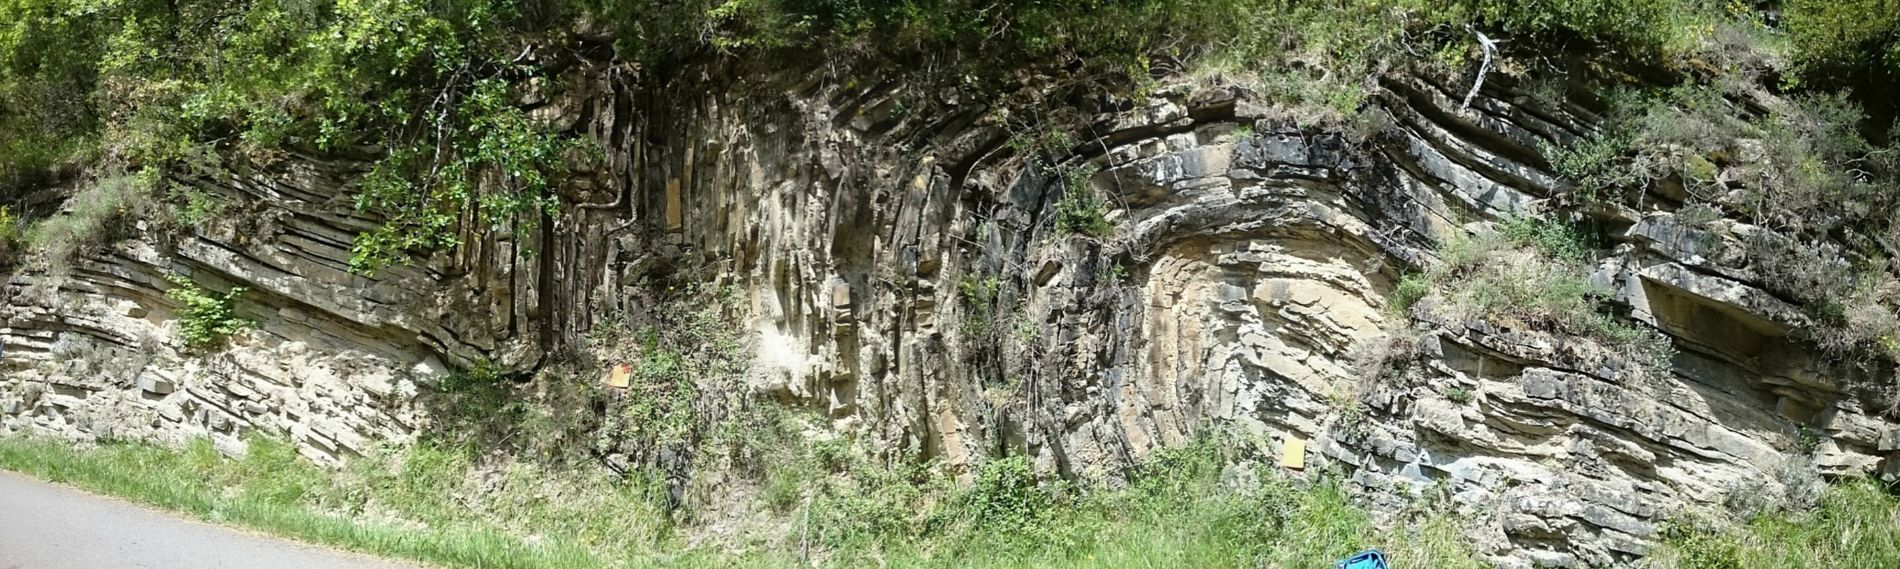
\includegraphics[width=0.8\textwidth]{Hecho1}\\
b & \includegraphics[width=0.8\textwidth]{Hecho2} \\
c & \includegraphics[width=0.8\textwidth]{Hecho3} \\
\end{tabular}
\caption{Folded turbidite lobes outcrop (a) and interpretation with the ``Full'' data set (b) and the ``sparse'' data set (c). 
Tangent and orientation data are shown as black lines and arrows.}
\label{fig:FLH2D}
\end{figure}

\todo[inline]{Add legend and full + sparse data sets}

The FLH2D data set (Fig. \ref{fig:FLH2D}) corresponds to a folded and faulted turbidite outcrop of approximately $16 \times 4$ m located in Aragues del Puerto, Spain. \todo[inline]{Add a location map} The layers correspond to Eocene turbidite lobes deposited in the Pyrenean foreland basin (Hecho Group) and then affected by north/south shortening. The interbedding of sandstone and shale beds is a source of mechanical heterogeneities which affected the localization of deformation during folding. Most of the shortening is accommodated by flexural slip of sandstone beds; shale beds follow a more ductile deformation between sandstone beds. The fold style (vergence, aperture) changes laterally and vertically, and probably results from variations in the relative thicknesses for the two main rock types. Some minor faults are visible and interpreted on the outcrop. The faults are provided as polygonal lines and triangulated surfaces extrapolated orthogonally 50 cm to the outcrop picture. The mesh resolution of the fault surfaces is approximately 15 cm. The sand lobes only display minor thickness variations at the scale of the outcrop, but some mild apparent thickness variation appears due to perspective. We chose to keep this artifact in the benchmark data set, as thickness variations management challenges have been documented for some implicit structural modeling methods \citep{Laurent2016EaPSL}. 

Nine horizons (H1 to H9) were interpreted on the image plane (XZ) as polygonal lines (Fig. \ref{fig:FLH2D}b) . For each of these lines, a random Y coordinate was sampled from a uniform law between -0.5 and 0.5 m to avoid singularities in the three-dimensional case. Some stratal traces and the associated slopes were also obtained by picking some segments parallel to the bedding on the surface. In addition to the ``full'' interpretation, a sparse interpretation is provided to test the ability of the methods to extrapolate away from the data (Fig. \ref{fig:FLH2D}c). This sparse data set only contains the faults and the horizons H1, H2, H4, H5, H7 and H9; only the subhorizontal part of H4 and H5 is provided. As a result, a significant data gap exists at the center of the outcrop between H7 and H2, where the observed layers are overall subvertical. 

The main goal of this data set is to test the ability of the structural modeling methods to honor conformable series affected by strong and laterally variable folds. 

\subsection{Claudius Data: carbonate mounds from NE Australia}

\begin{figure}

\centering\begin{tabular}{cc}
a & 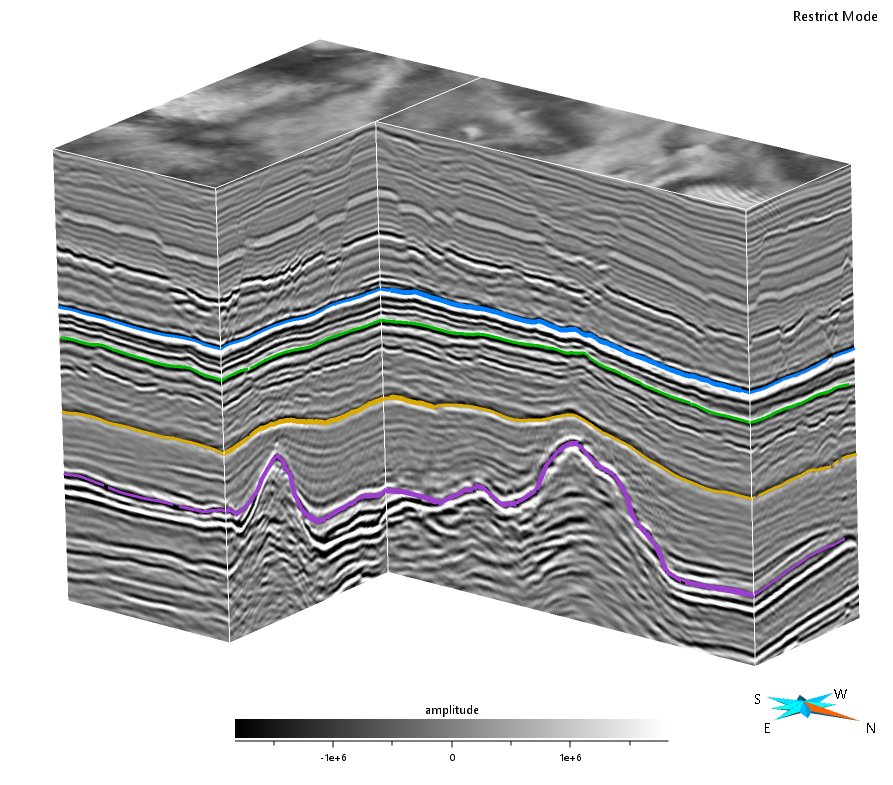
\includegraphics[width=0.7\textwidth,height=6cm]{Claudius}\\
b & 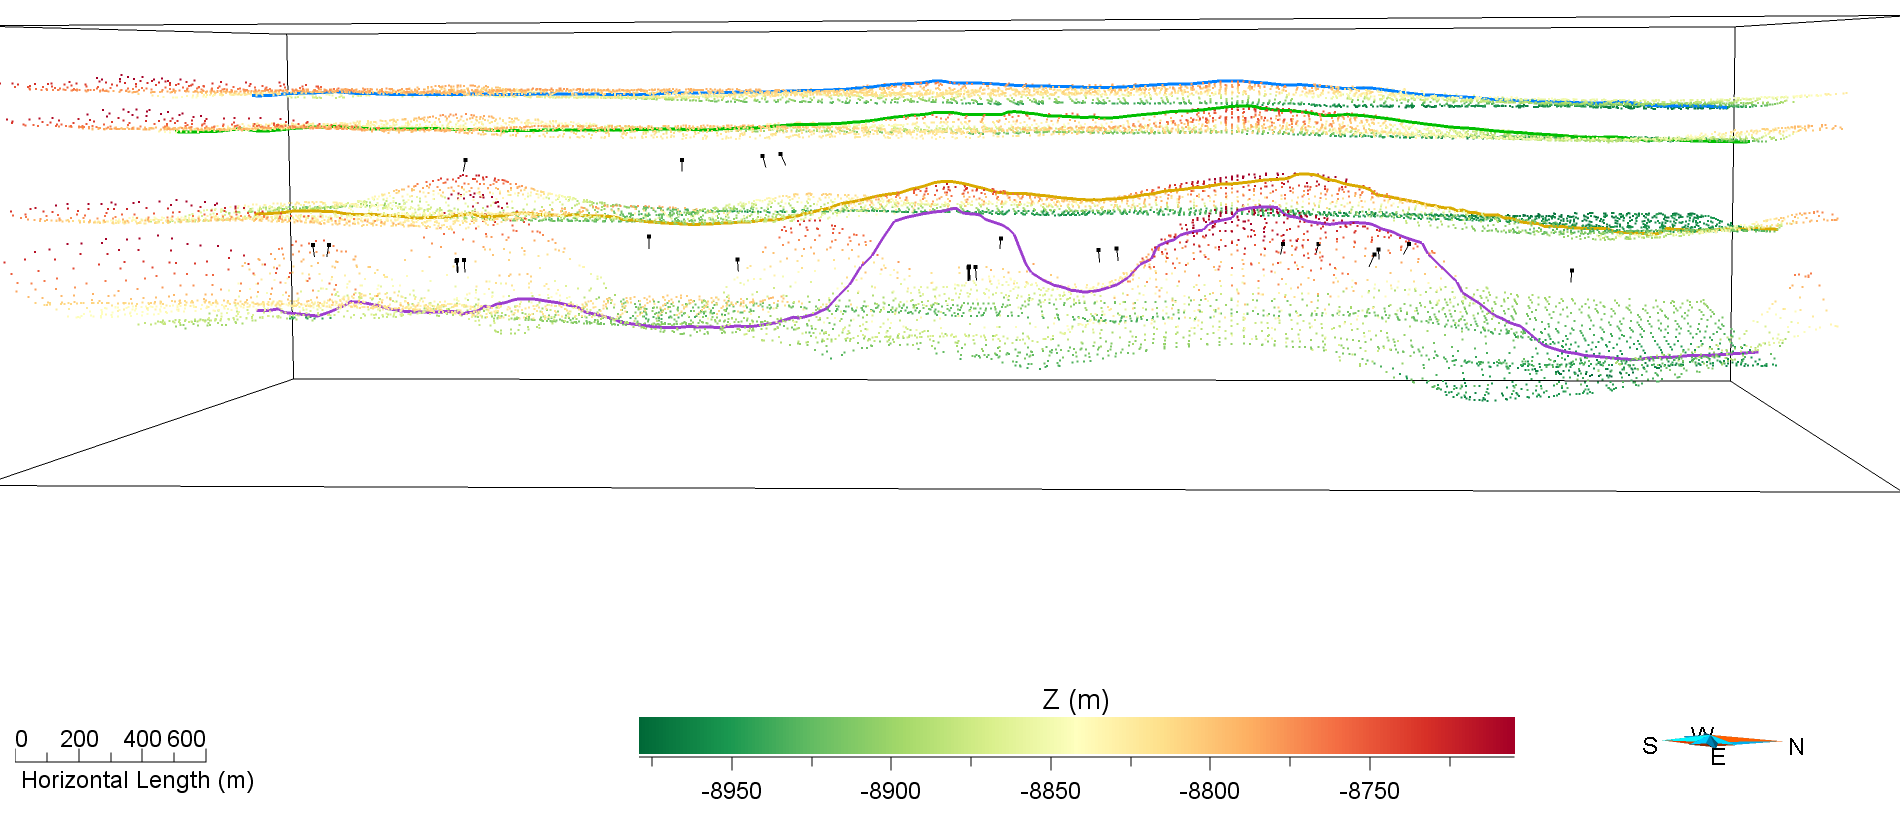
\includegraphics[width=0.8\textwidth]{Claudius1} \\
\end{tabular}
\caption{Interpreted stratigraphic series in the Claudius data set: sections (a) and points in side view (b). A is in blue, B in green, C in yellow and D in violet. In b, the Z Color scale bounds are set for each horizon. Orientation data (normal vectors) in black.}
\label{fig:ClaudiusData}
\end{figure}
\todo[inline]{Add legend and a figure with the reference surfaces and the data only + size details}


The second data set was taken from the offshore Carnarvon Basin, NW Australia. The Claudius area is imaged with a 3D seismic survey acquired by WesternGeco and provided by GeoScienceAustralia. We extracted a small stratigraphic section that displays several carbonate mounds and the associated slope and offshore deposits (Fig. \ref{fig:ClaudiusData}). We interpreted four main horizons named A to D. The most shallow horizon A is relatively flat, whereas D (the top of upper triassic carbonate build-ups) displays significant relief. The intermediate horizons B and C are slightly deformed maybe due to differential compaction. Overall, significant layer thickness variations exist between these stratigraphic surfaces. The detail of the seismic data set shows multiple slope deposits and onlaps, but at the scale of interest, we choose to consider here that the series is globally conformable. 

The main goal of this data set is to test the ability of implicit methods to model a stratigraphic series having strong thickness variations with one single continuous scalar field. 


\subsection{The Moureze 3D synthetic surface}

\begin{figure}
\centering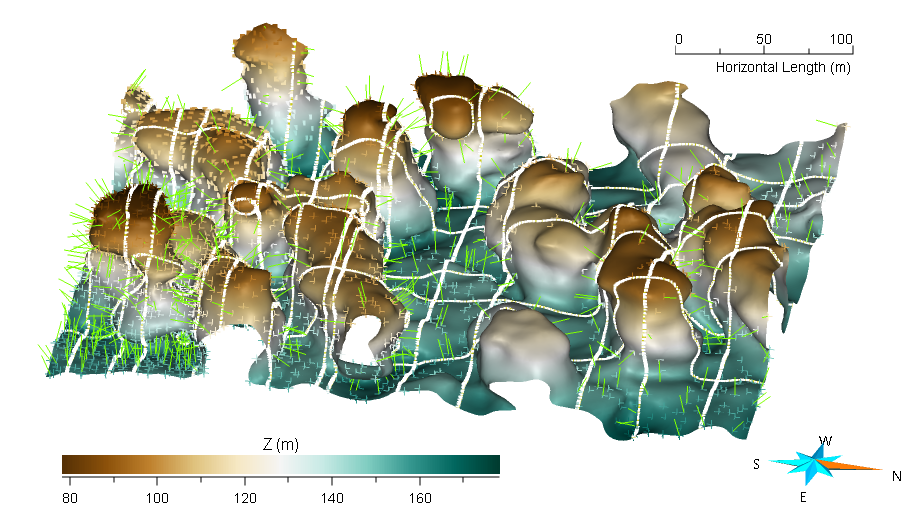
\includegraphics[width=\textwidth]{Moureze}
\caption{Synthetic complex surface generated by a perturbed distance field.}
\label{fig:Moureze}
\end{figure}
\todo[inline]{Add legend and a figure with the reference surfaces and the data only + size details}

To study the behavior of implicit interpolation methods for very complex structural geometries as encountered in salt tectonic studies and ore body delineation, we created a synthetic reference surface using the ODSIM (Object-Distance Simulation) method \citep{Henrion2010MG}. This method was initially introduced to model karsts and hydrothermal alteration bodies \citep{Henrion2008PEIGC,Rongier2014G} and was recently adapted to generate salt surfaces \citep{Clausolles20188ECE2}. In this study, we emulated a hydrothermal alteration body by defining a basement where several subvertical fractures are rooted. The fractures and the basement were simply defined by manual picking. The distance to the basement and the fracture set was then computed and perturbed by a spatially correlated random field (normal distribution of average 10 m and standard deviation equal to 36 m and Gaussian variogram model of a 36 m horizontal range (isotropic) and 20 m vertical range). Finally, the surface was obtained 
by thresholding (value of 28 m) the perturbed distance field and extracting the surface using Marching Cubes. Some additional cleaning was made to remove isolated bubbles and locally smooth and locally perturb (manually) the obtained geometry. This reference surface is made of one single connected component, but it has three handles.  

From this surface, we extracted two sets of seven E/W and thirteen N/S parallel cross-sections These sections only contain polygonal lines, some of which consist of several connected components. We also created an unstructured point set by decimating the nodes of the reference surface. The decimation strategy both performed by random sampling and by manual removal of nodes. The manual removal targeted some bumps so that only a very limited number of points remained to constrain the surface geometry. The resulting data points have a heterogeneous density in order to evaluate at once the ability of the reconstruction methods to retrieve the reference shape, both in the case of dense and sparse sampling conditions. A (randomly chosen) fraction of these nodes also provides information about the reference surface orientation. Both the section lines and the points are exactly on the reference surface, so data noise can be considered as negligible. 

\todo[inline]{
Discuss SIVAS (Pauline) or multi-phase fold (Eric). 

GC: The danger if there are too many data sets is that we will have too many results to present, making the paper complex. We can also propose other data sets and concentrate the results presentation on just a subset. }

%\subsection{Highly deformed series}

Options to be discussed: Maxelon's data base (https://doi.org/10.3929/ethz-a-004833149) and paper \citep{Maxelon2009C&G} could be a good test. and it would be nice to give credit to this seminal paper to bring in more geological concepts. The minus side is that some data preparation would be needed. 

We could also use some other challenging data sets in \citep{Laurent2016EaPSL,Grose2019JoSG,Sprague2005Ga}. 

Some remarks, to be discussed: 
\begin{enumerate}
\item As compared to the 2D cases, the challenge of a full 3D data set is that we don't have a picture to check results away from the data. the consequence is that we should decimate the data to keep some points as a test set. 

\item A criterion for selection is that the case study should be relatively simple to be illustrated in a paper. (even though it would be good to have a fairly large supplemental material with WebGL or some other 3D standard output). 

\item There should be at least a few contact data points so that all methods can be tried (and break again. It is good to break methods :-) 
This would help demonstrate the benefit of integrating S1, S2, etc. Possibly some optional inequality data could be used also. 

\end{enumerate}



\section{Methods}
\label{sec:methods}

Consider $S$ as the set of three-dimensional positions {x} where a three-dimensional scalar field $f(\mathbf{x})$ takes the value $f_S$: 

\begin{equation}
\label{eq:levelset}
  S = \{\mathbf{x} | f(\mathbf{x}) = f_S\}.
\end{equation}

In the general case of a spatially variable scalar field $f$ these positions form a two-dimensional manifold surface called iso-surface or level set, which represents geological surfaces in implicit methods. 

The expression (\ref{eq:levelset}) is easily extended to represent 
at once a stratigraphic series of $K$ conformable horizons 
$S_1, \ldots, S_K$ using different iso-values $f_1, \ldots, f_K$. 
In the following, we will call $f$ the stratigraphic function, which can be seen 
(in a chronostratigraphic sense) as a relative geological time \citep{Mallet2004MG,Lomask2006G,Wu2012G}.

In the presence of $N_k$ data points at positions $\{\mathbf{x}_1^k, \ldots, \mathbf{x}_{N_k}^k\}$ for the horizon $S_k$, all implicit surface interpolation methods start by forming the following system of equations: 

\begin{equation}
\label{eq:datasystem}
\begin{array}{r c l}
f(\mathbf{x}_1^1) & = & f_1 \\
\vdots & \vdots & \vdots \\
f(\mathbf{x}_{N_1}^1) & = & f_1 \\
\vdots & \vdots & \vdots \\
\vdots & \vdots & \vdots \\
f(\mathbf{x}_{N_1}^K) & = & f_K \\
\vdots & \vdots & \vdots \\
f(\mathbf{x}_{N_K}^K) & = & f_K \\
\end{array}
\end{equation}

Based on this principle, several methods have been proposed to compute a stratigraphic function at any spatial location $\mathbf{x}$. Essentially, these methods make different choices about:
 
\begin{enumerate}
\item \textbf{The handling of data}. For instance, dual cokriging \citep[DcK, ][]{Lajaunie1997MG,Chiles04OMSMP,Calcagno2008PEPI} performs a substitution in System (\ref{eq:datasystem}) so as to consider (unknown) increments of the scalar field as compared to one reference horizon instead of the absolute isovalues. This makes it possible to automatically compute the iso-values $f_k$ instead of using them as input to the interpolation problem, but it calls for at least one gradient data point to be included in the cokriging system. All methods can also take orientation data as input information, as the normal vector to the strata is collinear to the gradient $\nabla f$ of the stratigraphic function, see for instance \citet{Frank2007CG,Hillier2014MG}. Other possible data terms that have been integrated in the interpolation system relate for instance to fold axis \citep{MassiotGM2010,Hillier2014MG}, vergence \citep{Laurent2016EaPSL,Grose2017JSG} and thickness \citep{Laurent2016MG}.

\item The basis functions $\varphi_i(\mathbf{x})$ used to express $f(\mathbf{x})$ as a linear combination \citep[e.g., ][]{Renaudeau2019MG,Wellmann2018AiG}: 

\begin{equation}
\label{eq:basis}
  f(\mathbf{x}) = \sum_{i=1}^{N}{v_i\varphi_i(\mathbf{x})}.
\end{equation}

In radial basis function interpolation \citep[RBF, ][]{Cowan2002ASGMEM,Hillier2014MG} and dual co-kriging \citep[][]{Calcagno2008PEPI}, the basis functions are centered on the data points. In this case, $N$ refers to the total number of data points ($N = \sum_{k=1}^{K}{N_k}$). In discrete smooth interpolation \citep[DSI, ][]{Frank2007CG,Caumon2013GaRSITo,Souche20137ECEISE2,Irakarama2018EAGE}, $N$ refers to the number of nodes of the mesh used to approximate the solution. As recently discussed by \citet{Renaudeau2019MG}, these choices have a strong impact on the structure of the linear system that needs to be solved to evaluate the coefficients $v_i$ in Eq. (\ref{eq:basis}): a relatively small but dense system is formed in the case of RBF and DcK, whereas a larger but sparse system is formed in the case of DSI. Recently, \citet{Renaudeau2019MG} and \citet{Manchuk2019C&G} proposed to use moving least squares 

\item \textbf{The mathematical principle to ensure the uniqueness of the solution}. In kriging, this terms comes from the minimization of the estimation variance, which depends on the chosen variogram model. In dual kriging and RBF, the number of unknowns is such that the problem is well-posed, but the equivalence with thin plate energy has been made for spline basis functions. In DSI, the regularization is based on a minimization of the local variation of the gradient $\nabla f$ of the stratigraphic function $f$. This amounts to minimizing the deviations of the iso-surface from a plane. In general, all approaches implicitly or explicitly minimize some second order derivative of the scalar field, which may be the discrete Laplacian, the curvature energy or some other function of directional second derivatives. For more details, we refer to the review and discussion of \citet{Renaudeau2019MG}.

\end{enumerate}

\todo[inline]{Expand the method's descriptions. Create an table explaining the main parameters for each method}

\section{Results}\label{sec:results}

\todo[inline]{General idea: Put everyone's results on a shared server. Results mean: scalar fields (sampled on a fine Cartesian Grid) + iso-surfaces (triangulated) in some common format. Gocad ? OBJ ? We should probably decide very soon about the Cartesian grid extent and resolution for each data set.  }

To present the results, we plan to use a summary table with the main parameters retained for each method and each test case, and explain the rationale about the choice of these parameter values. The modeling results will be put on an open server, together with the scripts and software version information to allow the licensees of each considered software to reproduce the results. 

% \subsection {Consistency}

One of the first questions that want to consider is whether the reconstructed surfaces have the same topology as the reference surfaces. Indeed, implicit methods do not \textit{a priori} impose a particular topology for the implicit surfaces. This is a very interesting feature, for instance in the case of the Moureze data, as arbitrary topology can emerge from the data. However, bubbles should not appear when modeling layered strata, even in the case of sparse sampling or of strong thickness variations. 

% \subsection{Accuracy}

The second criterion concerns the accuracy of the interpolation. This should be a relatively easy case, as all methods generally have a parameter controlling the degree of data fit (e.g., the constraint weight in DSI or the variogram nugget effect in DcK). As not all methods use the same iso-values $f_k$, we plan to perform a projection of the points onto the reconstructed surfaces, and then check for possible bias (average of the signed distance) and error (variance of the deviation and maximum deviation corresponding to the Hausdorff distance). 

The third criterion will be to check the spatial forecasting ability, by checking the reconstructed surfaces against the reference geometries. This will be performed not only globally, but also in some targeted locations where data gaps were purposely introduced in the data set. In conjunction with the data accuracy, this should allow to test the ability of methods to predict some ``unseen'' features using the same data configuration, considering in particular the ability to extrapolate a horizon away from the data points laterally and orthogonally to the stratigraphy. Depending on the data configuration, it is likely that the regularization term might play a positive or adverse role there. In particular, when geological concepts and knowledge are incorporated as model parameters \citep[e.g.,][]{Laurent2016EaPSL,Grose2017JSG,Grose2018JGRSE,Grose2019JoSG} and when the choice of these model parameters is appropriate, it is possible to improve the predictive ability of models. Therefore, we also need to account for the number of method parameters and how they are infered and not just bluntly judge a method's performance based on RMS errors on some particular test data.  

Last, we also would like to provide some performance metrics about the various steps of the algorithms (domain construction, interpolation \textit{sensu stricto}, and isosurface visualization / extraction). A particular difficulty in this performance study will be to make sure that performance comparisons are sensible in spite of the probable use of different hardware configurations by the various co-authors. 

%\subsection{Performance}
 
\todo[inline]{Discuss about performance issues. This could be challenging, as everyone will run tests on a different machine, and codes have very different features (parallel or not, 2D or 3D). Scalability can be compared nonetheless by fitting a law regression between the number of points and the computational time. THis would call for everyone to apply the interpolation with decimated data sets (e.g. using 1/100, 1/50, 1/10, 1/5, 1/2 of the points)... The time ratio between model preparation (e.g., meshing), interpolation (solving the system) and visualization (marching cubes or the like) could also be considered. }


\section*{Conclusions}

We have proposed three data sets that can be used to assess the ability of implicit structural modeling methods to build relatively complex geological surfaces in the presence of sparse data. These data sets were designed to test both two-dimensional and three-dimensional implicit modeling codes. They are heterogeneous in size and in types of geological features, showing a highly conformable but strongly folded stratigraphic series, sedimentologically-controlled mini-basins involving fast changes of lateral stratigraphic thickness, and a complex fracture-controlled hydrothermal surface. 

We briefly reviewed the existing implicit modeling methods, which are currently being confronted to the benchmark data sets by the co-authors of this paper. Finally, we discussed about the criteria we intend to use to evaluate the benchmark results. 
Overall, we hope that these results will contribute to identifying avenues for further research in three-dimensional structural modeling, and that the proposed data can be used for testing future methods in the future. We welcome comments and suggestions for this work in progress. 

\section*{Acknowledgments}

This work was performed in the frame of the LOOP project (https://loop3d.org/) and the RING project (http://ring.georessources.univ-lorraine.fr/). We would like to thank for their support the industrial and academic sponsors of the RING-GOCAD Consortium managed by ASGA, and the LOOP project partners. We would also like to thank Geoscience Australia for providing the Claudius seismic data set and Emerson for the SKUA-GOCAD software used to prepare the data. 

% Set your bibliography file here (without .bib)
\bibliography{biblio}

\end{document}

%------------------------------------------
